\section{Optics Measurements}



% ===============================
%        Turn by Turn
% ===============================
\subsection{\todo{Turn by Turn}}





% ===============================
%         Chromaticity
% ===============================
\subsection{\review{Chromaticity}}

% --- Procedure ---
\subsubsection{Procedure}

Chromaticity measurements are typically performed by varying the RF frequency to induce a change of
momentum offset $\delta$, while measuring the tune.  The momentum offset $\delta$ being related to
the RF frequency and the momentum compaction factor $\alpha_c$:

\begin{equation}
    \delta = - \frac{1}{\alpha_c} \cdot \frac{\Delta f_{RF}}{f_{RF,nominal}}
    \label{eq:dpp_rf}
\end{equation}

Frequency steps of 20Hz every 30 secondes are usually taken to compromise between number of data
points, precision of the tune estimate, and duration of the measurement. Once beam losses,
registered by the BLMs are deemed too high, the frequency is reverted back to its nominal value in
larger steps. The same procedure is then re-applied in the negative. Figure
\ref{fig:measurements:rf_scan} shows a typical RF scan performed to measure chromaticity in the LHC.

\begin{figure}[H]
    \centering
    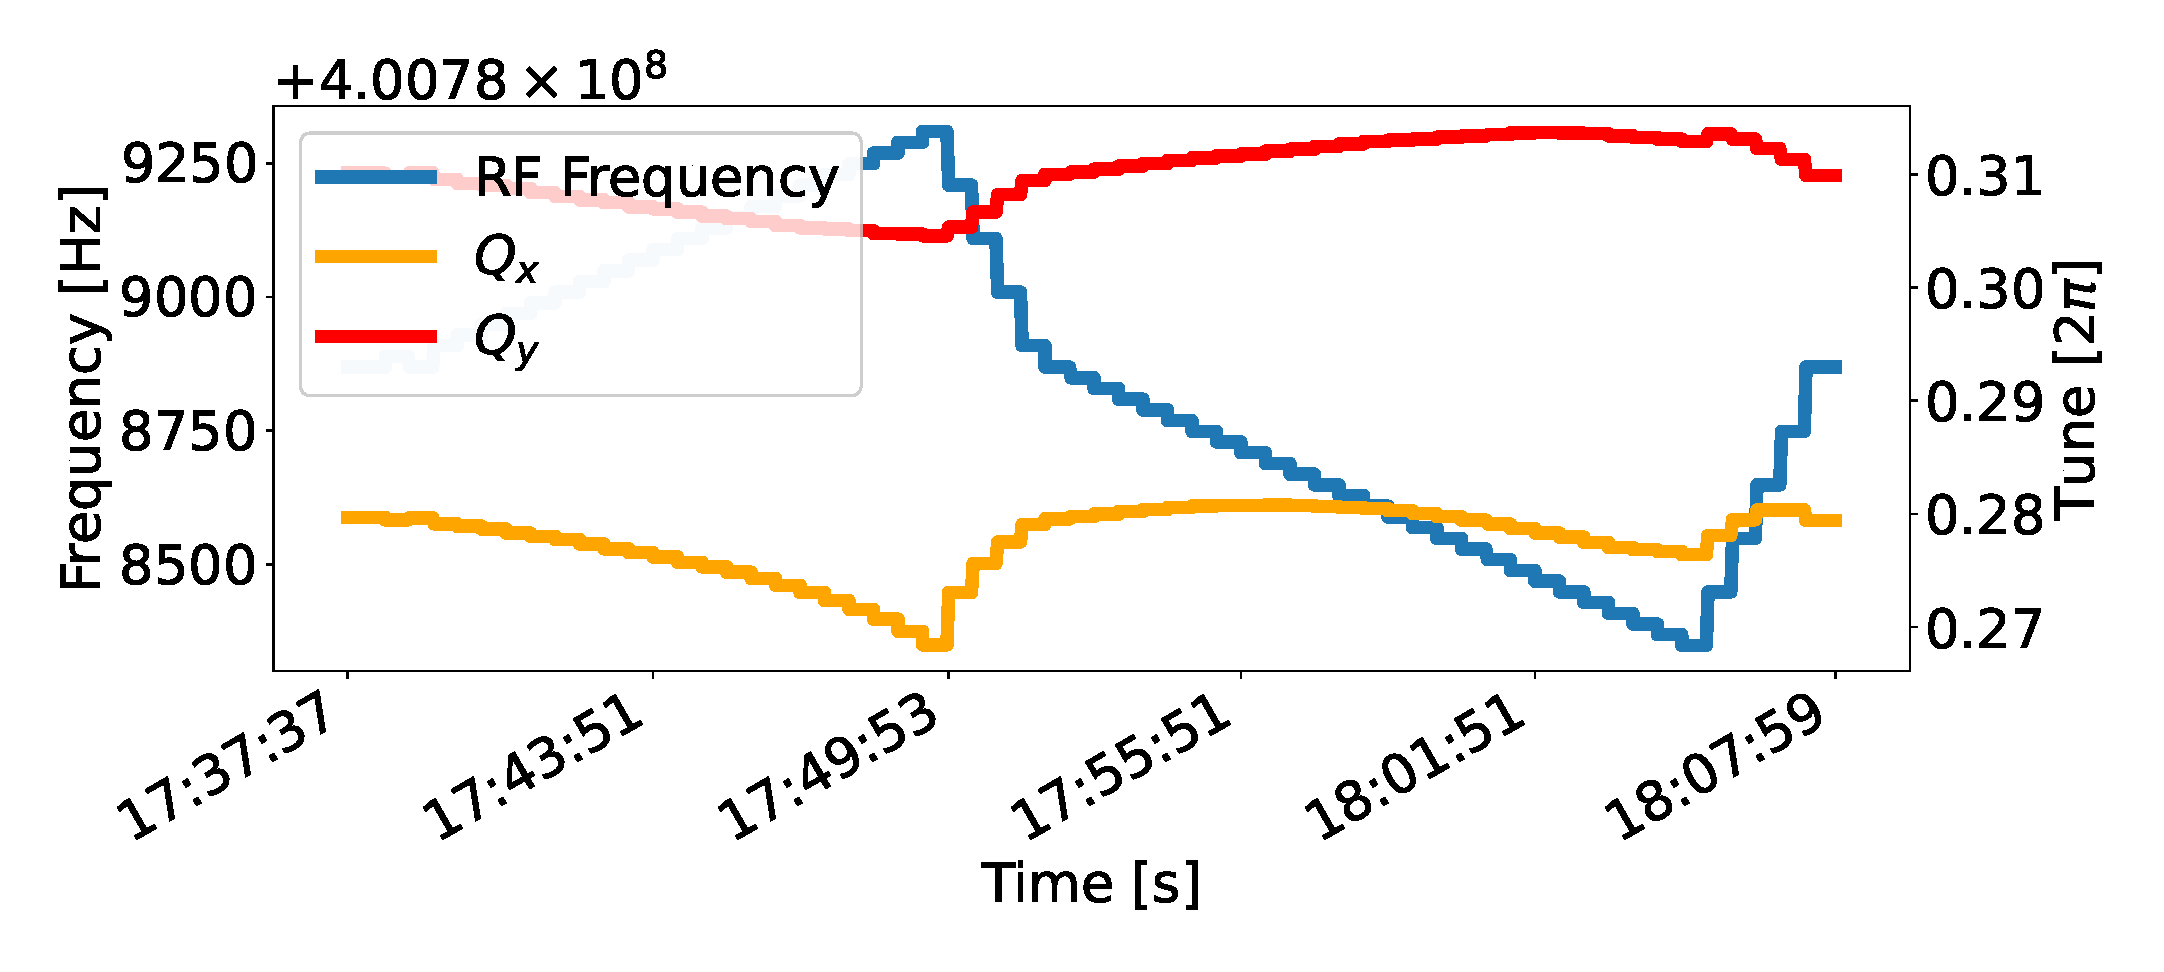
\includegraphics[width=1\textwidth]{images/rf_scan.pdf}
    \caption{Observation of the tune dependence on momentum offset, created by a shift of RF
             frequency.}
    \label{fig:measurements:rf_scan}
\end{figure}




% --- Analysis and Fit ---
\subsubsection{Analysis}

Once the tunes have been acquired and the momentum offset computed via Eq.~\eqref{eq:dpp_rf}, the
chromaticity function (see Eq.\eqref{eq:background_chromaticity}) can be used to fit the
measured data and retrieve each order.

As part of work for this thesis, a custom tool was developed, in order to ease such analysis of
chromaticity measurements. This tool, the Non-Linear Chromaticity
GUI~\cite{m_le_garrec_non-linear_2022}, is composed of several parts:

\begin{itemize}
    \tightlist
    \item Data extraction from CERN data servers (Timber, NXCALS)
    \item Tune cleaning and standard deviation calculation
    \item Chromaticity fit up to 7th order
    \item Corrections of chromaticity and resonance driving terms
\end{itemize}

Fits up to the third and fifth order using this tool can be seen in Fig.\ref{fig:chroma_gui}.

\begin{figure}[H]
    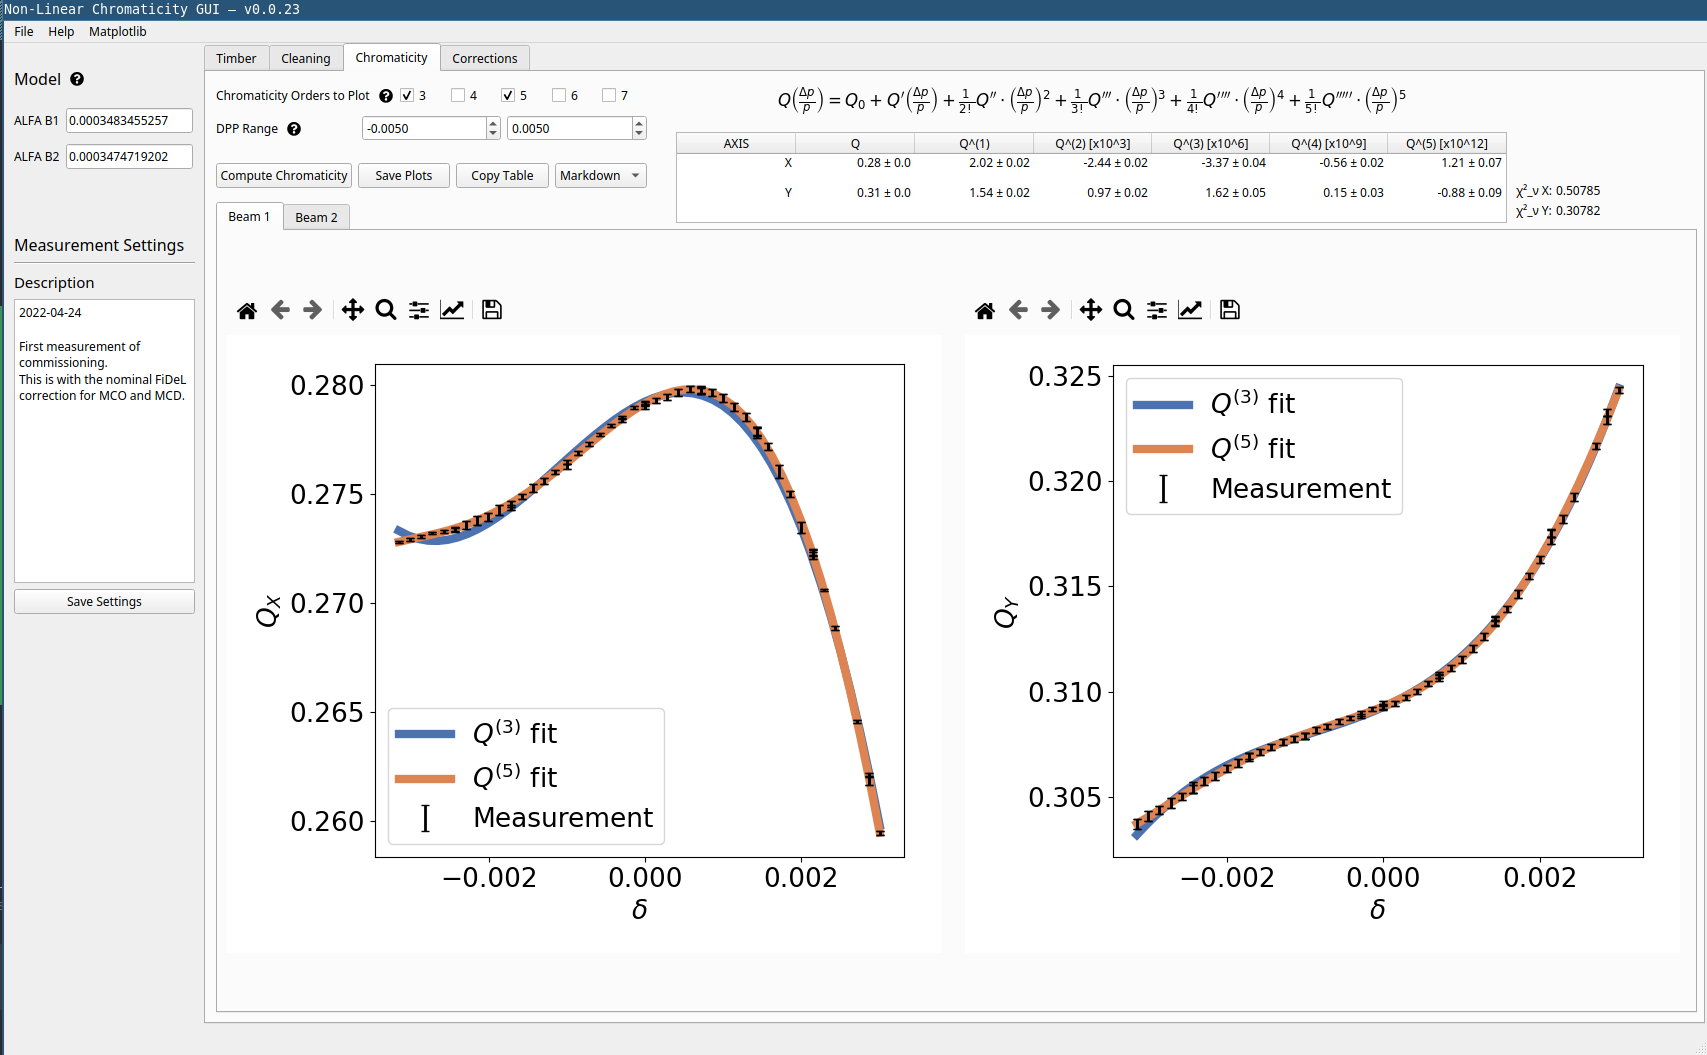
\includegraphics[width=\textwidth]{./images/chroma_gui.png}
    \caption{\textit{Non-Linear Chromaticity GUI} program, used to automatize chromaticity 
             analysis.}
    \label{fig:chroma_gui}
\end{figure}